\documentclass[a4paper]{article}
\usepackage{graphicx}
\usepackage{float}
\usepackage{pgfplots}
\pgfplotsset{compat=1.18}
\usepackage{listings}
\usepackage{enumitem}
\usepackage{cancel}
\usepackage{amsmath}
\usepackage{amssymb}
\usepackage{ebproof}
\usepackage{pgfplots}
\usepackage{tikz-cd}
\usepackage{forest}
\usetikzlibrary{decorations.pathreplacing} % for angle arc
\usetikzlibrary{angles, quotes, calc} % for drawing angles
\usepackage{color}   %May be necessary if you want to color links
\usepackage{hyperref}
\hypersetup{
    colorlinks=true, %set true if you want colored links
    linktoc=all,     %set to all if you want both sections and subsections linked
    linkcolor=black,  %choose some color if you want links to stand out
}


\usepackage{mathtools}
\DeclarePairedDelimiter\ceil{\lceil}{\rceil}
\DeclarePairedDelimiter\floor{\lfloor}{\rfloor}

\usepackage{xcolor}
\usepackage{tcolorbox}

% Define a custom tcolorbox environment for examples
\newtcolorbox{examplebox}[2][]{
  colback=blue!2!white,   % Background color
  colframe=blue!30!black, % Border color
  title=#2,          % Title of the box
  boxrule=0mm,          % Thickness of the border                % Rounded corners
  fonttitle=\bfseries,    % Title font style
  width=\textwidth,  
  #1 % Width of the box (adjustable)
}

\newtcolorbox{definition} {
  colback=green!5!white,   % Background color
  colframe=green!75!black, % Border color
  title=Definizione,          % Title of the box
  boxrule=0.5mm,          % Thickness of the border                % Rounded corners
  fonttitle=\bfseries,    % Title font style
  width=\textwidth,       % Width of the box (adjustable)
}



\definecolor{codegreen}{rgb}{0,0.6,0}
\definecolor{codegray}{rgb}{0.5,0.5,0.5}
\definecolor{codepurple}{rgb}{0.58,0,0.82}
\definecolor{backcolour}{rgb}{0.95,0.95,0.92}

\lstdefinestyle{mystyle}{
    backgroundcolor=\color{backcolour},   
    commentstyle=\color{codegreen},
    keywordstyle=\color{magenta},
    numberstyle=\tiny\color{codegray},
    stringstyle=\color{codepurple},
    basicstyle=\ttfamily\footnotesize,
    breakatwhitespace=false,         
    breaklines=true,                 
    captionpos=b,                    
    keepspaces=true,                 
    numbers=left,                    
    numbersep=5pt,                  
    showspaces=false,                
    showstringspaces=false,
    showtabs=false,                  
    tabsize=2
}

\lstset{style=mystyle}

\makeatletter
\renewcommand*\env@matrix[1][*\c@MaxMatrixCols c]{%
  \hskip -\arraycolsep
  \let\@ifnextchar\new@ifnextchar
  \array{#1}}
\makeatother
\usepackage{tikz}
\usepackage{booktabs}
\title{Algoritmi}
\author{Università di Verona\\Imbriani Paolo -VR500437\\Professor Roberto Segala}

\begin{document}

\begin{figure}
    \centering
    \includegraphics[width=0.3\textwidth]{UniversityofVerona.png}
    \label{fig:centered-image}
\end{figure}

\maketitle 

\pagebreak

\tableofcontents

\pagebreak

\section{Introduzione}


Ci sono diverse definizioni di 'algoritmo' ma quella più semplice per definirlo è una sequenza di istruzioni volta a risolvere un problema. In maniera più semplice, possiamo definirlo come una ricetta. Le ricette sono delle istruzioni per creare dei piatti: queste istruzioni sono precise tuttavia possono avere anche delle varianti. Il problema non è trovare la ricetta, ma capire quale sia quella gisuta da utilizzare in base al problema posto. 
\\\\
In questo corso impararemo come \textit{decidere}. Studiare i diversi approcci e il metodo migliore per affrontare un problema.
Capiremo come confrontare gli algoritmi fra di loro.

\subsection{Complessità}

Classifichiamo gli algoritmi in base alla loro complessità ovvero quanto tempo ci mettono per essere completati. Il nostro obiettivo è quello non di misurare il tempo in sè (poiché può dipendere dal tipo di macchina che utilizziamo) che impiega un programma a finire ma piuttosto capire il numero di istruzioni elementari che vengono impiegate per risolvere il problema.
\\\\
La complessità non è un numero bensì una funzione, poiché mappa la dimensione del problema in numero di istruzioni da eseguire. Per esempio, quando si parla di dimensione di una matrice ci si viene più comodo vedere il numero di colonne e righe piuttosto che contare il numero di elementi all'interno della matrice. La dimensione del problema è un insieme di oggetti, tipicamente un insieme di numeri che ci permette di avere un idea chiara di capire quanto sia grande il problema. Se riusciamo a misurarlo bene, potremmo facilitarci la vita nel risolvere il problema. 

\subsection{Complessità dei costrutti e ordini di grandezza}

È doveroso stare attenti a cosa moltiplichiamo: se moltiplichiamo due vettori, il numero di operazioni da eseguire è esattamente $n$. Mentre se fossero orgnanizzate in matrici quadrate con lunghezza del lato $\sqrt{n}$ la sua complessità andrebbe ad aumentare a $O(n\sqrt{n})$.
Come si rappresentano le istruzioni di un programma?
Se sono in serie:
\[\begin{matrix}
  I_1 & c_1(n)\\
  I_2 & c_2(n)\\
  \vdots\\
  I_l & c_l(n)
\end{matrix}\]
Dove la complessità totale allora sarà:
\[\sum_{i=1}^l c_i(n)\]
oppure all'interno di un costrutto \textbf{if-else:}
\[\begin{matrix}
  \text{if cond} & c_{\text{cond}}(n)\\
  I_2 & c_1(n)\\
  \text{else}\\
  I_l & c_2(n)
\end{matrix}\]
In questo caso, come faccio a sapere la complessità totale di questi istruzioni? Per capirlo, studiamo il caso nel \textit{worst case scenario} ovvero nel caso peggiore. A volte vengono mostrati anche i casi migliore ma di solito si calcola il tempo peggiore. Quindi ci interessa specialmente il \textit{limite superiore} dell'algoritmo, quindi piuttosto che dire che la complessità è esattamente \textbf{uguale} questo numero, invece noi diremo che è \textbf{minore o uguale} del numero calcolato.

\[C(n) = c_{\text{cond}}(n) + max(c_1(n), c_2(n))\]
Mentre per un while loop? 
\[\begin{matrix}
    \text{while cond} & c_{cond}(n)\\
    I & c_0(n)
\end{matrix}\]
Sia $m$ limite superiore numero di iterazioni che esegue l'algoritmo. La complessità di questo algoritmo quindi sarà:
\[C(n) = c_{cond}(n) + m(c_{cond}(n) + c_0(n))\]
Proviamo ora a calcolare la molteplicazioni tra matrici.
Siano due matrici $A$ e $B$ rispettivamente con dimensione $n$ x $m$ e $m$ x $l$.
\begin{lstlisting}
For i <- 1 to n
    For j <- 1 to l
        C[i][j] <- 0
        For k <- 1 to m
            C[i][j] += A[i][j] * B[k][j]
\end{lstlisting}
Avere un risultato del tipo $5m + 1$ (riguardo il for più interno) è inutile perché non ci da informazioni realmente utili sulla complessità dell'algoritmo. 
Ad ogni modo contando tutti i for, avremo un risultato del tipo:

\[n(5ml + 4l + 2) + n + 1 = 5nml + 4nl + 3n + 1\]
Ci sono alcuni elementi in questa operazioni che non influiscono realmente sul risultato finale. Indi per cui, possiamo anche ometterlo all'interno del calcolo della complessità di un algoritmo.
In realtà ciò che ci interessa realmente nel risultato finale è:
\[5\colorbox{yellow}{\textbf{nml}}+ 4nl + 3n + 1\]
Infatti $nml$ è capace di dirci tutto sulla complessità dell'algoritmo e da cosa dipende. 
Quando si parla di ordine di grandezza si parla in realtà del comportamento asintotico della funzione calcolata.
\begin{definition}
\[f \in O(g)  \Longleftrightarrow \exists c > 0, \,\, \exists \overline{n}, \,\, \forall n \ge \overline{n} \, | \, f(n) \le cg(n)\]
\end{definition}
\begin{figure}[H]
    \centering
    \caption{$f \in O(g)$}
\begin{tikzpicture}
    \begin{axis}[
        axis lines = middle,
        xlabel = $x$,
        ylabel = {$\textcolor{blue}{f(n)}, \textcolor{red}{cg(n)}$},
        legend pos=north west,
        domain=2:8,
        samples=200,
        xmin=2, xmax=8, ymin=-5, ymax=30,
        width=12cm,
        height=8cm
    ]
        % Plot f(x) = exp(x) / 5
        \addplot[color=red, thick] {(exp(x))/5};
        
        % Plot g(x) = (30*ln(x)) / (sin(x) + 3)
        \addplot[color=blue, thick] {(30*ln(x))/(sin(deg(x)) + 3)};
        
        % Add a vertical line at the intersection point
        \addplot[mark=none, black, dashed, thick] coordinates {(4.8, 0) (4.8, 24)};
        \node at (axis cs:4.2,25) [anchor=west] {$\overline{n}$};
        
    \end{axis}
\end{tikzpicture}
\end{figure}

\begin{definition}
  \[f \in \Omega(g) \Longleftrightarrow \exists c > 0, \,\, \exists \overline{n}, \,\, \forall n \ge \overline{n} \, | \, f(n) \ge cg(n)\]  
  Che rispettivamente è l'inverso della funzione O grande.
\end{definition}

\begin{figure}[H]
    \centering
    \caption{$f \in \Omega(g)$}
\begin{tikzpicture}
    \begin{axis}[
        axis lines = middle,
        xlabel = $x$,
        ylabel = {$\textcolor{blue}{f(n)}, \textcolor{red}{cg(n)}$},
        legend pos=north west,
        domain=2:8,
        samples=200,
        xmin=2, xmax=8, ymin=-5, ymax=30,
        width=12cm,
        height=8cm
    ]
        % Plot f(x) = exp(x) / 5
        \addplot[color=blue, thick] {(exp(x))/5};
        
        % Plot g(x) = (30*ln(x)) / (sin(x) + 3)
        \addplot[color=red, thick] {(30*ln(x))/(sin(deg(x)) + 3)};
        
        % Add a vertical line at the intersection point
        \addplot[mark=none, black, dashed, thick] coordinates {(4.8, 0) (4.8, 24)};
        \node at (axis cs:4.2,25) [anchor=west] {$\overline{n}$};
        
    \end{axis}
\end{tikzpicture}
\end{figure}
\begin{definition}
  \[f \in \Theta(g) \Longleftrightarrow f \in O(g)  \, \wedge \, f \in \Omega(g)\]  
\end{definition}

\begin{figure}[H]
    \centering
    \caption{$f \in \Theta(g)$}
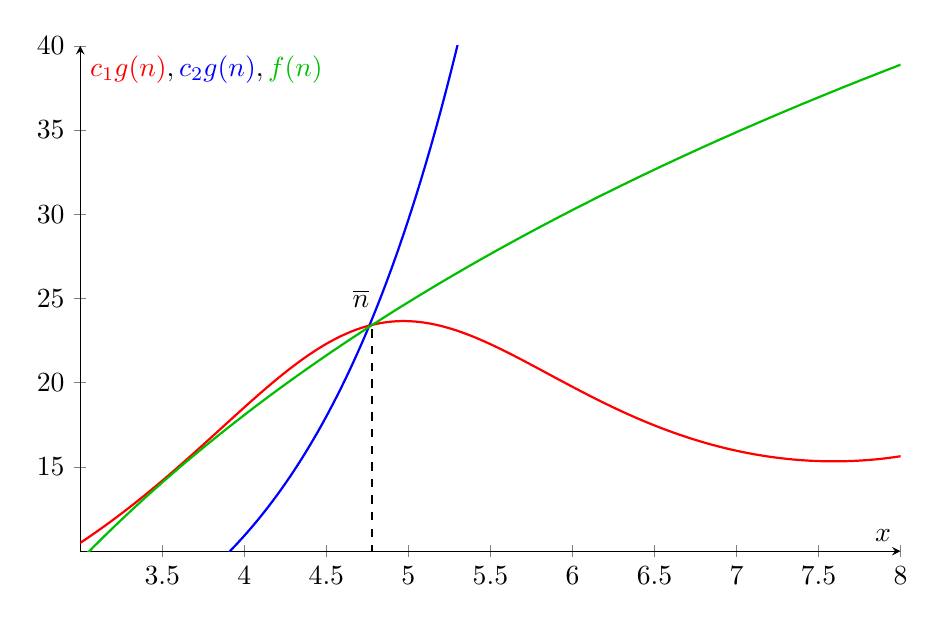
\begin{tikzpicture}
    \begin{axis}[
        axis lines = middle,
        xlabel = $x$,
        ylabel = {$\textcolor{red}{c_1g(n)}, \textcolor{blue}{c_2g(n)}, \textcolor{green!75!black}{f(n)}$},
        legend pos=north west,
        domain=2:8,
        samples=200,
        xmin=3, xmax=8, ymin=10, ymax=40,
        width=12cm,
        height=8cm
    ]
        \addplot[color=blue, thick] {(exp(x))/5};
        \addplot[color=red, thick] {(30*ln(x))/(sin(deg(x)) + 3)};
        \addplot[color=green!75!black, thick] {30*ln(x) - 23.5};

        
        % Add a vertical line at the intersection point
        \addplot[mark=none, black, dashed, thick] coordinates {(4.78, 0) (4.78, 23.65)};
        \node at (axis cs:4.6,25) [anchor=west] {$\overline{n}$};
        
    \end{axis}
\end{tikzpicture}
\end{figure}



\begin{examplebox}{Esempio 1}
Questa affermazione vale?
\[n \in O(2n)\]
Sì, perché esiste un $c$ che soddisfa $n \le c2n$.\\\\
Quest'altra affermazione vale?
\[2n \in O(n)\]
Sì perché esiste un $c$ che soddisfa $2n \le 2n$.
\end{examplebox}
\begin{examplebox}{Esempio 2}
Questa affermazione vale?
\[f \in O(g) \Longleftrightarrow g \in \Omega(g)\]
Proviamo a dimostrare. Sappiamo che esiste un $c$ e $\overline{n}$ tale che \(\forall n > \overline{n} \; f(n) \le cg(n)\). Isoliamo la g:
\[g(n) \ge \frac{1}{c} f(n)\]
Esiste quindi un c' che soddisfa la disuguaglianza. 
\[c' = \frac{1}{c}\]
\end{examplebox}
\begin{examplebox}{Esempio 3}

\[f_1 \in O(g), 
f_2 \in O(g) \Longrightarrow f_1 + f_2 \in O(g)
\]
Dobbiamo dimostrare che esiste $c_1$ e $c_2$, $\overline{n}_1$ e $\overline{n}_2$ tali che:
\[\forall n > \overline{n}_1 \; | \; f_1(n) \le c_1g(n)\]
\[\forall n > \overline{n}_2 \; | \; f_2(n) \le c_2g(n)\]
Quindi
\[\overline{n} = max(\overline{n}_1, \overline{n}_2)\]
\[f_1(n) + f_2(n) \le (c_1 + c_2)g(n)\]
    
\end{examplebox}

\begin{examplebox}{Esempio 4}
    \[f_1 \in O(g_1), f_2 \in O(g_2) \; | \; f_1f_2 \in O(g_1g_2)\]
Quindi esiste $c_1$ e $c_2$, $\overline{n}_1$ e $\overline{n}_2$ tali che:
\[\forall n > \overline{n}_1 \; | \; f_1(n) \le c_1g(n)\]
\[\forall n > \overline{n}_2 \; | \; f_2(n) \le c_2g(n)\]
\[f_1(n)f_2(n) \le c_1g_1(n)c_2g_2(n)\]
\[f_1(n)f_2(n) \le c_1c_2g_1(n)g_2(n)\]
Quindi:
 \[c = c_1c_2\] \[\overline{n} = max(\overline{n}_1, \overline{n}_2)\]
\end{examplebox}

\subsection{Ordini di grandezza per le funzioni}

L'algoritmo di ricerca $A$ termina entro n. Immaginiamo che l'algoritmo A sia il seguente:
\begin{lstlisting}
For i <- 0 to length(a) - 1
    if a[i] = x
        ret i
ret -1
\end{lstlisting}
Capiamo che la sua complessità è uguale a:
\[A \in O(n)\]
Per appurarci che la stima di complessità sia accurata dobbiamo controllare che $A \in \Omega(g)$ vuol dire che esiste uno schema di input tale per cui se $g(n)$ è il numero di passi necessari per risolvere l'istanza $n$, allora $g \in \Omega(f)$. Se riusciamo a fare questo allora $g \in \Theta(f)$ e quindi possiamo dire che la stima è accurata.
\\\\
$P \in O(f)$ vuol dire che il problema $P$ riesco a risolvere in tempo $f$. Supponiamo per assurdo che esista un algoritmo riesca a capire se l'elemento si trova nell'array o no. Possiamo capire velocemente che per contraddizione, essendo che esiste almeno un elemento dove l'algoritmo non ha guardato, siamo certi del malfunzionamento dell'algoritmo e quindi non è vero che esiste una stima di complessità più bassa di $f$.


\section{Analisi di algoritmi}

Ora andiamo ad affrontare i tipi di algoritmi che si definiscono di "ordinamento". 
\begin{definition}
\textbf{Input}: Sequenza $(a_1, ..., a_n)$ di oggetti su cui è definita una relazione di ordinamento (in questo caso ordinamento per confronti).
\\\\
\textbf{Output}: Permutazione $(a_1', ..., a_n')$ di $(a_1, ..., a_n)$ t.c. $\forall \, i > j, \; \; a_i' \le a_j'$.
\end{definition}
Andiamo ora a vedere i diversi tipi di algoritmi di ordinamento.

\subsection{insertion$\_$sort (A)}

In questo caso la $j$ sarà chiamata variabile "invariante" ovvero che mantiene una proprietà che continua a valere nel run-time dell'algoritmo. In questo caso, la $j$ è invariante perchè tutti gli oggetti "a sinistra" di essa saranno considerati già ordinati. (Parte da 2 perché abbiamo deciso che la posizione all'interno dell'array parte da 1).

\begin{lstlisting}
for j <- 2 to length[A]
    key <- A[j]
    i <- j - 1
    while i > 0 and A[i] > key
        A[i+1] <- A[i]
        i--
    a[i+1] <- key
\end{lstlisting}
Ora dobbiamo capire quale sia la complessità di questo algoritmo. Se le cose vanno bene, l'algoritmo potrebbe terminare in $O(n)$. Tuttavia, seppur giusto, non è preciso. Infatti, nel peggiore dei casi, l'algoritmo termina in $O(n^2)$. Infatti il caso peggiore di input che mi può arrivare è un array ordinato al contrario con complessità uguale a:
\[1 + 2 + 3 + ... + n = \frac{n(n+1)}{2} \in \Theta(n^2)\]
\textit{Questo algoritmo, quanto spazio di memoria usa in più rispetto allo spazio occupato dai dati? }
\\\\
Lo spazio di memoria di questo algoritmo rimane costante a prescindere dalla dimensione del problema. Un algoritmo del genere si dice che \textit{\textbf{ordina in loco}} se la quantità di memoria extra è costante. Si parla di \textit{\textbf{stabilità}} di un algoritmo di ordinamento quando l'ordine relativo di elementi uguali non viene scambiato dall'algoritmo. Quindi:
\[\text{Se } a_i = a_j \, i < j, \text{mantiene l'ordinamento}\]


\section{Concetto di "Divide et impera"}

\subsection{Fattoriale e funzioni ricorsive}

\begin{lstlisting}
Fatt(n) 
    if n = 0
        ret 1
    else
        ret n * fatt(n - 1)
\end{lstlisting}

L'argomento della funzione ci fa capire la complessità dell'algoritmo:
\[
  T(n) = \begin{cases}
    1 & \text{se } n = 0 \\
    T(n - 1) + 1 & \text{se } n > 0
  \end{cases}
\] 
Con problemi ricorsivi si avrà una complessità con funzioni definite ricorsivamente.
Questo si risolve induttivamente:
\[
  \begin{aligned}
    T(n) & = 1 + T(n-1)\\
         & = 1 + 1 + T(n-2)\\
         & = 1 + 1 + 1 + T(n-3)\\
         & = \underbrace{1 + 1 + \ldots + 1}_{i} + T(n-i)\\
  \end{aligned}
\] 
La condizione di uscita è: \( n-i = 0 \quad n = i \) 
\[
\begin{aligned}
         & = \underbrace{1 + 1 + \ldots + 1}_{n} + T(n-n)\\
         & = n + 1 = \Theta(n)
\end{aligned}
\] 
Questo si chiama passaggio iterativo.

\begin{examplebox}{Esempio 1}
  \[
    T(n) = 2T\left(\floor*{\frac{n}{2}}\right) + n
  \] 
  Questa funzione si può riscrivere come:
  \[
  T(n) = \begin{cases}
    \text{Costante} & \text{se } n < a \\
    2T\left(\floor*{\frac{n}{2}}\right) + n & \text{se } n \ge a
  \end{cases}
  \] 

  \vspace{1em}
  \noindent
  Se la complessità fosse già data bisognerebbe soltanto verificare se è corretta.
  Usando il metodo di sostituzione:
  \[
    T(n) = cn \log n
  \] 
  sostituiamo nella funzione di partenza:
  \[
    \begin{aligned}
      T(n)  & = 2T\left(\floor*{\frac{n}{2}}\right) + n\\
            & \le 2c\left(\floor*{\frac{n}{2}}\right) \log \floor*{\frac{n}{2}} + n\\
            & \le \cancel{2} c \frac{n}{\cancel{2}} \log \frac{n}{2} + n\\
            & = cn \log n - cn \log 2 + n\\
            & \stackrel{?}{\le} cn \log n \quad \text{se } n- cn \log 2 \le 0\\
    \end{aligned}
  \] 
  \[
    c \ge \frac{n}{n \log 2} = \frac{1}{\log 2}
  \] 
  Il metodo di sostituzione dice che quando si arriva ad avere una disequazione
  corrispondente all'ipotesi, allora la soluzione è corretta se soddisfa una certa ipotesi.
\end{examplebox}

\begin{examplebox}{Esempio 2}
  \[
    T(n) = T\left(\floor*{\frac{n}{2}}\right) + T\left(\ceil*{\frac{n}{2}}\right) + 1 \quad \in O(n)
  \] 
  \[
  T(n) \le cn
  \] 
  \[
  \begin{aligned}
    T(n) & = T\left(\floor*{\frac{n}{2}}\right) + T\left(\ceil*{\frac{n}{2}}\right) + 1\\
         & \le c\left(\floor*{\frac{n}{2}}\right) + c\left(\ceil*{\frac{n}{2}}\right) + 1\\
         & = c \left( \left\lfloor \frac{n}{2} \right\rfloor + \left\lceil \frac{n}{2} \right\rceil  \right) + 1\\
         & = cn + 1 \stackrel{?}{\le} cn
  \end{aligned}
  \] 
  Il metodo utilizzato non funziona perchè rimane l'1 e non si può togliere in alcun modo.
  Per risolvere questo problema bisogna risolverne uno più forte:
  \[
  T(n) \le cn - b
  \] 
  \[
  \begin{aligned}
    T(n) & = T\left(\floor*{\frac{n}{2}}\right) + T\left(\ceil*{\frac{n}{2}}\right) + 1\\
         & \le c\left(\floor*{\frac{n}{2}}\right) -b + c\left(\ceil*{\frac{n}{2}}\right) -b + 1\\
         & = c \left( \left\lfloor \frac{n}{2} \right\rfloor + \left\lceil \frac{n}{2} \right\rceil  \right) - 2b + 1\\
         & = cn - 2b + 1 \stackrel{?}{\le} cn - b\\
         & = \underbrace{cn - b} + \underbrace{1 - b}_{\le 0} \le cn - b \quad \text{se } b \ge 1\\
  \end{aligned}
  \] 
  Se la proprietà vale per questo problema allora vale anche per il problema iniziale
  perchè è meno forte.
\end{examplebox}

\begin{examplebox}{Esempio 3}
  \[
    \begin{aligned}
      T(n) & = 3T \left( \left\lfloor \frac{n}{4} \right\rfloor \right) + n\\
           & = n + 3T \left( \left\lfloor \frac{n}{4} \right\rfloor \right)\\
           & = n + 3 \left( \left\lfloor \frac{n}{4} \right\rfloor + 3T 
           \left( \left\lfloor \frac{\left\lfloor \frac{n}{4} \right\rfloor}{4} \right\rfloor
           \right)  \right)\\
           & = n + 3 \left\lfloor \frac{n}{4} \right\rfloor + 3^2 T 
           \left( \left\lfloor \frac{n}{4^2} \right\rfloor \right)\\
           & \le n + 3 \left\lfloor \frac{n}{4} \right\rfloor + 3^2 
           \left( \left\lfloor \frac{n}{4^2} \right\rfloor + 3T \left( 
           \left\lfloor \frac{\left\lfloor \frac{n}{4^2} \right\rfloor}{4} \right\rfloor
           \right)  \right) \\
           & = n + 3 \left\lfloor \frac{n}{4} \right\rfloor + 3^2
           \left\lfloor \frac{n}{4^2} \right\rfloor + 3^3 T
           \left( \left\lfloor \frac{n}{4^3} \right\rfloor \right) \\
           & = n + 3 \left\lfloor \frac{n}{4} \right\rfloor + \ldots + 3^{i-1}
           \left\lfloor \frac{n}{4^{i-1}} \right\rfloor + 3^i T
           \left( \left\lfloor \frac{n}{4^i} \right\rfloor \right) 
    \end{aligned}
  \]


  Per trovare il caso base poniamo l'argomento di T molto piccolo:
  \[
    \begin{aligned}
      \frac{n}{4^i} & < 1\\
      4^i & > n\\
      i & > \log_4 n
    \end{aligned}
  \] 
  L'equazione diventa:
  \[
    \begin{aligned}
      & \le n + 3 \left\lfloor \frac{n}{4} \right\rfloor + \ldots + 3^{\log_4 n - 1}
      \left\lfloor \frac{n}{4^{\log_4 n - 1}} \right\rfloor + 3^{\log_4 n} c\\
    \end{aligned}
  \] 


  Si può togliere l'approssimazione per difetto per ottenere un maggiorante:
  \[
  \begin{aligned}
    & \le n \left( 1 + \frac{3}{4} + \left( \frac{3}{4} \right)^2 + \ldots +
    \left( \frac{3}{4} \right)^{\log_4 n-1} \right) + 3^{\log_4 n} c\\
    & \le n \left( \sum_{i=0}^{\infty} \left( \frac{3}{4} \right)^i \right) + c 3^{\log_4 n}\\
  \end{aligned}
  \] 
    \end{examplebox}
\begin{examplebox}{}
  Per capire l'ordine di grandezza di \( 3^{\log_4 n} \) si può scrivere come:
  \[
    3^{\log_4 n} = n^{\left( \log_n 3^{\log_4 n} \right) } = n^{\log_4 n \cdot \log_n 3}
    = n^{\log_4 3}
  \] 
  Quindi la complessità è:
  \[
  \begin{aligned}
    & = O(n) + O(n^{\log_4 3})\\
  \end{aligned}
  \] 
  Si ha che una funzione è uguale al termine noto della funzione originale e l'altra
  che è uguale al logaritmo dei termini noti. Se usassimo delle variabili uscirebbe:
  \[
    \begin{aligned}
      T(n) & = a T \left( \left\lfloor \frac{n}{b} \right\rfloor \right) + f(n)\\
           & = O(f(n)) + O(n^{\log_b a})
    \end{aligned}
  \] 
\end{examplebox}



\subsection{Master Theorem o Teorema dell'esperto}

Data una relazione di occorrenza di questa forma:

\[T(n) = a T \left( \left\lfloor \frac{n}{b} \right\rfloor \right) + f(n)\]

Distinguiamo tre casi:

\begin{enumerate}
    \item \[f(n) \in O(n^{\log_ba - \epsilon}) \Longrightarrow T(n) \in \Theta(n^{\log_ba})\]
    \item \[f(n) \in \Theta(n^{\log_ba}) \Longrightarrow T(n) \in \Theta(f(n)\log n)\]
    \item \[f(n) \in \Omega(n^{\log_ba} + \epsilon) \Longrightarrow T(n) \in \Theta(f(n))\]
\end{enumerate}

\begin{examplebox}{Esempio 1}
    \[T(n) = 9T\left(\frac{n}{3}\right) + n\]
    \[a = 3, b = 3, f(n) = n\]
    Basta che trovo un $\epsilon$ che mi dia $n$.
    \[n^{\log_b a} = n^{\log_3 9} = n^2 * n^{-\frac{1}{2}}\]
    In questo caso $\epsilon = n^{-\frac{1}{2}}$ e ci troviamo nel \textbf{PRIMO CASO} e la soluzione è $T(n) \in \Theta(n^2)$.
\end{examplebox}

\begin{examplebox}{Esempio 2}
       \[T(n) = T\left(\frac{2n}{3}\right) + 1\]
    \[a = 1, b = \frac{3}{2}, f(n) = n^0\]
    \[n^{\log_b a} = n^{\log_{\frac{3}{2}} 1} = n^0\]
    Ci troviamo nel \textbf{SECONDO CASO} e la soluzione è $T(n) \in \Theta(\log n))$
\end{examplebox}

\begin{examplebox}{Esempio 3}
    \[T(n) = 3T\left(\frac{n}{4}\right) + n \log n\]
       \[a = 3, b = 4, f(n) = n \log n\]
       Ci troviamo nel \textbf{TERZO CASO} quindi basta qualsiasi valore di $\epsilon$ basta che sia contenuto tra $\log_3 4 \le \epsilon \le 1$. La soluzione è $T(n) \in \Theta(n\log n)$.
\end{examplebox}

\begin{examplebox}{Esempio 4} 
    \[T(n) = 2T\left(\frac{n}{2}\right) + n \log n\]
       \[a = 2, b = 2, f(n) = n \log n\]
    \[n\log n \in \Omega(n^{1 + \stackrel{?}{\epsilon}}) \]
    \[\log n \in \Omega(n^\epsilon) \text{ NON VALE}\]
    Poiché un logaritmo è sempre più piccolo di un polinomio.
    Questo è un caso dove il teorema \textit{non} si applica
\end{examplebox}


\subsection{Merge Sort (A, n)}

Questo algoritmo di ordinamento \textit{ricorsivo} utilizza il concetto di \textit{divide et impera}. 

Concettualmente, un merge sort funziona come segue:

\begin{enumerate}
    \item \textbf{Dividi} l'array non ordinato in n sottoarray, ognuno contenente un elemento (un array di un elemento è considerato ordinato).
    \item \textbf{Unisci} ripetutamente i sottoarray per produrre nuovi sottoarray ordinati finché non ne rimane solo uno. Questo sarà l'array ordinato.
\end{enumerate}
La sua complessità considerando il merge con complessità lineare risulta:
\[T(n) = 2T\left(\frac{n}{2}\right) + n\]
Utilizzando il \textbf{Master Theorem} e cadendo del \textit{secondo caso} possiamo confermare che il risultato è:
\[= \Theta(n \log n)\]

\begin{lstlisting}[language=Scala]
// A e' l'array mentre p ed r sono rispettivamente l'indice di partenza e di arrivo 
mergeSort(A, p, r) // O(n log n)
    if (p < r) 
        q <- floor((p+r)/2)
        mergeSort(A, p, q)
        mergeSort(A, q+1, r)
        merge(A, p, q, r)
\end{lstlisting}
\begin{lstlisting}[language=Scala]
merge(A, p, q, r)
    i <- 1
    j <- p
    k <- q+1
    // Ordina gli elementi di A in B
    // O il lato sinistro ha finito 
    while(j <= q or k <= r) // O(n)
        if j <= q and (k > r or A[j] <= A[k])
            B[i] <- A[j]  
            j++
        else
            B[i] <- A[k] 
            k++
        i++
    // Copia gli elementi di B in A
    for i <- 1 to r-p+1  // O(n)
        A[p+i-1] <- B[i]
\end{lstlisting}
L'algoritmo è \textbf{stabile} poiché non vengono scambiati gli elementi uguali. Tuttavia non ordina \textbf{in loco} poiché utilizza uno spazio di memoria aggiuntivo.
\subsection{Heap}
L'Heap è un albero semicompleto (ogni nodo ha 2 figli ad ogni livello tranne l'ultimo  che è completo solo fino ad un certo unto) in cui i nodi contengono oggetti con relazione di ordinamento.\\\\
\textbf{\textit{Proprietà Heap:}}

\[\forall \text{ nodo, il contenuto è } \ge \text{ del contenuto dei figli}\]

\begin{figure}[H]
    \centering
    
    \begin{forest}
for tree={
    draw, % Disegna i nodi
    circle, % Forma dei nodi
    minimum size=1.5em, % Dimensione minima dei nodi
    inner sep=1pt, % Spaziatura interna dei nodi
    s sep=1.5cm % Spaziatura verticale tra i livelli
}
  [16, edge label={node[right, xshift=7pt] {1}}
    [14, edge label={node[above, yshift=7pt] {2}}
      [8, edge label={node[above, yshift=7pt] {4}}
        [1, edge label={node[above, yshift=7pt] {8}}]
        [2, edge label={node[above, yshift=7pt] {9}}]
      ]
      [9, edge label={node[above, yshift=7pt] {5}}
        [3, edge label={node[right, xshift=7pt] {10}}]
      ]
    ]
    [10, edge label={node[above, yshift=7pt] {3}}
      [2, edge label={node[above, yshift=7pt] {6}}]
      [3, edge label={node[above, yshift=7pt] {7}}]
    ]
  ]
\end{forest}    
    \label{fig:enter-label}
\end{figure}
La complessità dell'algoritmo è in base al numero di livelli dell'albero.\\\\
$\longrightarrow$ albero con $n$ livelli: 
\[\# \text{Nodi} = 2^0 + 2^1 + 2^2 + ... + 2^{n - 1} = \frac{1 - 2^n}{1-2} = 2^n - 1\]
$\longrightarrow$ albero con $n$ nodi: 
\[\# \text{Livelli} = \log_2n\]
\[\#\text{Foglie} = \frac{n}{2}\]
Le foglie di un albero sono la metà dei nodi dell'albero.

\begin{lstlisting}[language=Scala]
extractMax(H) // O(log n)
    h[1] <- H[H.heap_size()]
    H.heap_size()--
    heapify(H, 1)
\end{lstlisting}

\begin{lstlisting}[language=Scala]
heapify(H, 1) // O(log n)
    l <- left[i] // 
    r <- right[i] 
    if(l < h.heap_size() AND H[l] > H[i]
        largest <- l
    else
        largest <- i
    if m <= h.heap_size() and H[r] > H[largest]
        largest <- r
    if largest != i
        swap(H[i], H[largest])
        heapify(H, largest)
\end{lstlisting}
Creare uno heap da un array:
\begin{lstlisting}[language=Scala]
buildHeap(A) 
    A.heap_size() <- length[A]
        for i <- length[A]/2 down to 1
            heapify(A, i)
\end{lstlisting}
Immagino tutte le foglie come heap con un solo nodo. L'indice del primo nodo che non è heap corrisponde a $\frac{length(A)}{2}$ su questo allora chiamo \texttt{heapify}.

\pagebreak

\subsection{Heapsort}
\begin{lstlisting}[language=Scala]
HeapSort(A) // O(n log n)
    buildHeap(A)
    for i <- length(A) to 1
        scambia(A[1], A[i])
        heapsize(A)--
        heapify(a, i)
\end{lstlisting}
L'Heap Sort è un algoritmo che lavora \textbf{in loco} tuttavia non è \textbf{stabile}. Tuttavia riusciamo a fare una stima migliore e più corretta? 
\[n \log i = \sum_{i=1}^n \log i = \log \prod_{i=1}^n i = \log n! = \Theta(\log n^n) = \Theta(n \log n)\]
In questo caso, essere accurati non aiuta, ma abbiamo avuto la certezza che non esiste una stima migliore.
\subsection{Quicksort}
Come funziona l'algoritmo?
\begin{enumerate}
    \item Dividi prima l'array in due parti. (Partizione)
    \item  Devi essere sicuro che tutti gli elementi di sinistra siano $\le$ di quelli di destra. Ricorsivamente ordina la parte sinistra e la parte destra.
    \item A questo punto l'array è ordinato.
\end{enumerate}

\begin{lstlisting}[language=Scala]
quickSort(A, p, r)
    if (p < r) 
        q <- partition(a, p, r)
        quickSort(A, p, q)
        quickSort(A, q+1, r)
\end{lstlisting}

\begin{lstlisting}[language=Scala]
partition(A, p, r) // O(n)
    x <- A[p] // Elemento Perno
    i <- p-1
    k <- r+1
    while true
        repeat j-- until a[j] <= x        
        repeat i++ until a[i] >= x
        if i < j
            scambia(a[i], a[j])
        else
            ret j
\end{lstlisting}
Scegliamo un elemento a caso in base a quello comparato rispetto all'elemento perno tale che:
\[sx \le perno \le dx\]
Questo algoritmo non è \textbf{stabile} ma lavora \textbf{in loco}.
La sua complessità?
\[T(n) = T(\text{partition}) + T(q) + T(n-q)\]
Se il quicksort è perfettamente diviso in due, allora la sua complessità è $O(n \log n)$.
Se invece l'array è già ordinato la sua equazione di ricorrenza sarà:
\[= n + T(1) + T(n-1) = \colorbox{yellow!50!white}{$\Theta(n^2)$}\]
Tuttavia non ci aspettiamo che questo caso sia frequente e quindin nella stra grande maggioranza dei casi allora:
\[T(n) = n + T(cn) + T((1-c)n)\]
Un equazione di questo tipo sappiamo che ha come complessità $\Theta(n \log n)$.
\begin{lstlisting}[language=Scala]
rand_Partition(A, p, r)
    i <- rand(p .. r) // Ora l'elemento perno e' un elemento a caso
    scambio(A[p], A[i]
    ret partition(A, p, r)
\end{lstlisting}

\begin{align*}
    T(n) &= n + \frac{1}{n}(T(1) + T(n-1) + \frac{1}{n}(T(2) + (T-2)) + \; \dots \; + \\ 
    & \frac{1}{n}(T(n-2) + T(2)) + \frac{1}{n}(T(n-1) + T(1) = \\
    &= n + \frac{1}{n} \sum_{i}(T(i) + T(n-i))\\
    &= n + \frac{2}{n} \sum_{i} T(i) \in \colorbox{green!30!white}{$O(n \log n$)}
\end{align*}
Qualsiasi algoritmo che\textit{ lavora per confronti }deve fare almeno $O(n \log n)$. 

\subsection{Counting Sort}
Tuttavia possiamo trovare algoritmi che come tempo di esecuzione hanno tempo lineare. Come? Non lavorando a \textbf{confronti}. 
\\\\
Come ordinare $n$ numeri con valori da 1 a $k$?
\begin{lstlisting}[language=Scala]
countingSort(A, k)
    for i <- 1 to k 
        C[i] <- 0
    for j <- 1 to len(A)
        C[A[j]]++
    for i <- 2 to k
        C[i] <- C[i-1]+C[i]
    for j <- len(A) down to 1
        B[C[A[j]]] <- a[j]
        C[A[J]]--
\end{lstlisting}
La complessità di questo algoritmo è $O(n + k)$ dove $n$ è la lunghezza dell'array e $k$ e il range di valori.
\end{document}
 